\documentclass[a4paper]{article}
\usepackage[a4paper,top=2cm,bottom=2cm,left=1cm,right=1cm,marginparwidth=1.75cm]{geometry}
% \usepackage[spanish]{babel}
% \selectlanguage{spanish}
% \usepackage[utf8]{inputenc}
% \usepackage[T1]{fontenc}
% \usepackage[spanish]{babel}

% \usepackage[T1]{fontenc}
\usepackage{graphicx} %Paquete para usar imagenes
\usepackage{listings}
\usepackage{xcolor}
\usepackage{tcolorbox}

\definecolor{background}{HTML}{E7EBF4}
\definecolor{bg}{HTML}{1a1b26}
\definecolor{fg}{HTML}{a9b1d6}
\definecolor{comment}{HTML}{848cb5}
\definecolor{cyan}{HTML}{82aaff}
\definecolor{orange}{HTML}{ff9e64}
\definecolor{yellow}{HTML}{e9d78e}
\definecolor{purple}{HTML}{c792ea}
\definecolor{green}{HTML}{7fdbca}
\definecolor{numbers}{HTML}{9854f1}
\definecolor{keyword}{HTML}{9854f1}

\lstset{
    showspaces=false, % Evita mostrar espacios en blanco como ␣
    showstringspaces=false,
    inputencoding=utf8,
    extendedchars=true,
    literate=%
    {á}{{\'a}}1
    {é}{{\'e}}1
    {í}{{\'i}}1
    {ó}{{\'o}}1
    {ú}{{\'u}}1
    {ñ}{{\~n}}1
}
\lstdefinestyle{mystyle}{
    language=Python,
    basicstyle=\ttfamily,
    keywordstyle=\color{keyword},
    commentstyle=\color{comment},
    numbers=none,
    numberstyle=\tiny\color{numbers},
    frame=none,
    breaklines=true,
    % showstringspaces=false
    xleftmargin=0mm,
    xrightmargin=0mm,
}

\lstset{style=mystyle}

\newtcolorbox{mycodebox}[1][]{
    arc=17pt,  % Radio de las esquinas redondeadas
    colback=background,  % Color de fondo del cuadro
    boxrule=0.5pt,  % Grosor de la línea del cuadro
    colframe=background,
    width=0.8\textwidth,   % Anchura del cuadro
    % height=5cm,            % Altura del cuadro
    % breakable,
    #1  % Otras opciones personalizadas que puedas necesitar
}


\newtcolorbox{mycodeboxl}[1][]{
    arc=7pt,  % Radio de las esquinas redondeadas
    colback=background,  % Color de fondo del cuadro
    boxrule=0.5pt,  % Grosor de la línea del cuadro
    colframe=background,
    width=0.94\textwidth,   % Anchura del cuadro
    % height=5cm,            % Altura del cuadro
    % breakable,
    #1  % Otras opciones personalizadas que puedas necesitar
}

% Documento
\begin{document}
\newgeometry{left=3cm,right=3cm,top=2cm,bottom=2cm}
\begin{titlepage}

%--------------- Nuevo comendo de linea ----------------->
\newcommand{\linea}{\rule{\linewidth}{0.7mm}} 
\center
%--------------- Universidad, facultad y carrera ----------------->
\textbf{\Large UNIVERSIDAD NACIONAL DE SAN ANTONIO ABAD DEL CUSCO}\\[0.2cm]
\textbf{\Large FACULTAD DE INGENIERÍA ELÉCTRICA, ELECTRÓNICA,INFORMÁTICA Y MECÁNICA}\\[0.2cm]
\textbf{\Large INGENIERÍA INFORMÁTICA Y DE SISTEMAS\\[0.6cm]}

%--------------- Escudos png ----------------->

\includegraphics[width=8cm]{src/escudo-unsaac.png}
\vfill

%--------------- Tema ----------------->
\linea
\\[0.3cm]
% \vfill
\textbf{\LARGE Guía de Laboratorio 4 - Traslación}\\[0.2cm]
\linea \\
\vfill

%--------------- Integrantes ----------------->
\textit{\Large Alumno:}\\
%Integrantes del grupo
    \textbf{\large Ian Logan Will Quispe Ventura}\\
    \textit{211359}\\
    % \vfill

%--------------- Profesor y curso ----------------->
\vspace{0.3cm}
    \textit{\Large Docente:}\\
    \textbf{\large Hector Eduardo Ugarte Rojas}\\
\vspace{0.5cm}
    \textit{\Large Curso:}\\
    \textbf{\large Computación Gráfica}\\
    \vfill

\vspace{0.4cm}
    \textbf{\Large Cusco - Perú }\\
    \textbf{\large 2023 - II }\\
    \newpage
    \end{titlepage}

\restoregeometry
\newpage
% •·•·•·•·•·•••·•·•·•·•·•·•·•·•·•·•·•·•·•·•·•·•·•·•·•·•.,..,
% \section{Funcionamiento del algoritmo DDA}

\Large{\textbf{Algoritmo de Traslación de una Linea en Python}}\\[-0.4cm]
\begin{center}
\begin{mycodebox}
\begin{lstlisting}
from OpenGL.GL import *
from OpenGL.GLUT import *
from OpenGL.GLU import *

def trasladaLinea(P, T):
    # Dibuja la línea original
    glColor3f(0.8, 0.26, 1.0)
    glBegin(GL_LINES)
    glVertex2f(P[0][0], P[0][1])
    glVertex2f(P[1][0], P[1][1])
    glEnd()
    # Calcula las coordenadas de traslación
    P[0][0] += T[0]
    P[0][1] += T[1]
    P[1][0] += T[0]
    P[1][1] += T[1]
    glColor3f (0.5 , 0.3 , 0.9)
    # Dibuja la línea trasladada
    glBegin(GL_LINES)
    glVertex2f(P[0][0], P[0][1])
    glVertex2f(P[1][0], P[1][1])
    glEnd()
    glFlush()

def display():
    P = [[150, 80], [320, 380]] 
    T = [100, 60]
    glClear(GL_COLOR_BUFFER_BIT) 
    trasladaLinea(P, T) 
    glFlush() 

def myinit():
    glClearColor (0.9, 0.92, 0.95, 1.0)
    glMatrixMode(GL_PROJECTION) 
    glLoadIdentity() 
    gluOrtho2D(0.0, 499.0, 0.0, 499.0)  
\end{lstlisting}
\end{mycodebox}
\end{center}

\begin{center}
\begin{mycodebox}
\begin{lstlisting}
# Función principal
def main():
    # Inicialización de GLUT estándar
    glutInit(sys.argv)
    glutInitDisplayMode(GLUT_SINGLE | GLUT_RGB)
    glutInitWindowSize(500, 500)  
    glutInitWindowPosition(0, 0)  
    glutCreateWindow("Traslación de líneas") 
    glutDisplayFunc(display) 
    myinit() 
    glutMainLoop() 

# Llama a la función principal
if __name__ == "__main__":
    main()
\end{lstlisting}
\end{mycodebox}
\end{center}
Gráfico generado 
\begin{center}
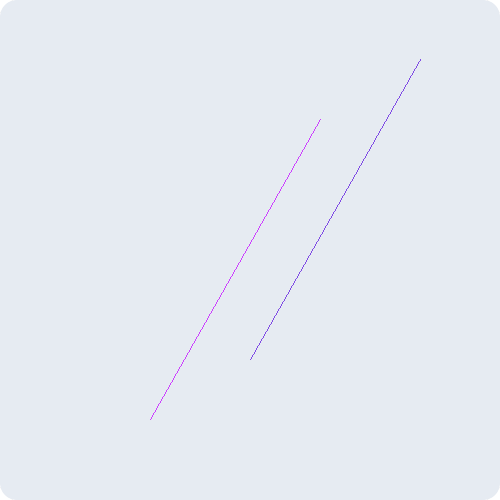
\includegraphics[width=13cm]{src/1.png}
\end{center}
\newpage
\Large{\textbf{Algoritmo de Traslación de un Rectángulo en Python}}\\[-0.4cm]
\begin{center}
\begin{mycodebox}
\begin{lstlisting}
from OpenGL.GL import *
from OpenGL.GLUT import *
from OpenGL.GLU import *

def trasladaRectangulo(P, T):
    glColor3f(0.8, 0.26, 1.0)
    glBegin(GL_LINES)
    # -- IZQUIERDA
    glVertex2f(P[0][0], P[0][1])
    glVertex2f(P[0][0], P[1][1])
    # -- ARRIBA
    glVertex2f(P[0][0], P[1][1])
    glVertex2f(P[1][0], P[1][1])
    # -- DERECHA
    glVertex2f(P[1][0], P[1][1])
    glVertex2f(P[1][0], P[0][1])
    # -- ABAJO
    glVertex2f(P[1][0], P[0][1])
    glVertex2f(P[0][0], P[0][1])
    glEnd()

    # Calcula las coordenadas de traslación
    P[0][0] += T[0]
    P[0][1] += T[1]
    P[1][0] += T[0]
    P[1][1] += T[1] 

    glColor3f (0.5 , 0.3 , 0.9)
    # Dibuja el rectángulo trasladado
    glBegin(GL_LINES)
    glVertex2f(P[0][0], P[0][1])
    glVertex2f(P[0][0], P[1][1])
    # -- ARRIBA
    glVertex2f(P[0][0], P[1][1])
    glVertex2f(P[1][0], P[1][1])

\end{lstlisting}
\end{mycodebox}
\end{center}

\begin{center}
\begin{mycodebox}
\begin{lstlisting}
    # -- DERECHA
    glVertex2f(P[1][0], P[1][1])
    glVertex2f(P[1][0], P[0][1])
    # -- ABAJO
    glVertex2f(P[1][0], P[0][1])
    glVertex2f(P[0][0], P[0][1])
    glEnd()
\end{lstlisting}
\end{mycodebox}
\end{center}
% \newpage
Gráfico generado 
\begin{center}
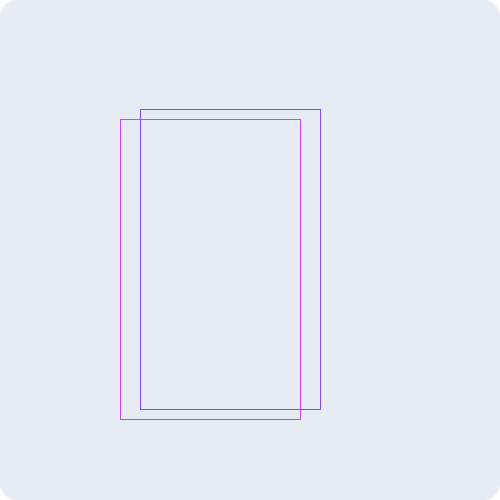
\includegraphics[width=16cm]{src/2.png}
\end{center}
\newpage


\Large{\textbf{Algoritmo de Traslación de un circulo en Python}}\\[-0.4cm]
\begin{center}
\begin{mycodebox}
\begin{lstlisting}
from OpenGL.GL import *
from OpenGL.GLUT import *
from OpenGL.GLU import *
import math

# Configuración inicial
width, height = 500, 450
r = 0.4
change = 0
p = [[0, 0] for _ in range(6)]

# Función para dibujar círculos
def draw(tx, ty):
    global r
    glBegin(GL_LINE_LOOP)
    for i in range(1200):
        theta = 2 * math.pi * i / 1200
        x1 = r * math.cos(theta) + tx
        y1 = r * math.sin(theta) + ty
        glVertex2f(x1, y1)
    glEnd()

# Función de visualización
def display():
    global width, height, r, change, p
    glClear(GL_COLOR_BUFFER_BIT | GL_DEPTH_BUFFER_BIT)
    glClearColor(0.9, 0.92, 0.95, 1.0) 
    glColor3f(0.8, 0.26, 1.0)  
    glMatrixMode(GL_MODELVIEW)
    j = 0
    change = 1 - change
    glBegin(GL_LINE_LOOP)
    for i in range(1200):
        theta = 2 * math.pi * i / 1200
        x1 = r * math.cos(theta)
        y1 = r * math.sin(theta) 
\end{lstlisting}
\end{mycodebox}
\end{center}

\begin{center}
\begin{mycodebox}
\begin{lstlisting}
        glVertex2f(x1, y1)
        if i in [100, 300, 500, 700, 900, 1100] and change == 0:
            p[j] = [x1, y1]
            j += 1
    glEnd()
    if change == 0:
        glColor3f(0.5, 0.3, 0.9)  
        for i in range(6):
            draw(p[i][0], p[i][1])
    glutSwapBuffers()

# Función principal
def main():
    glutInit()
    glutInitDisplayMode(GLUT_DOUBLE | GLUT_RGB | GLUT_DEPTH)
    glutInitWindowSize(width, height)
    glutCreateWindow("circles".encode("ascii"))
    glutDisplayFunc(display)
    glutIdleFunc(display)
    glutMainLoop()

main()
\end{lstlisting}
\end{mycodebox}
\end{center}
\newpage
Gráfico generado 
\begin{center}
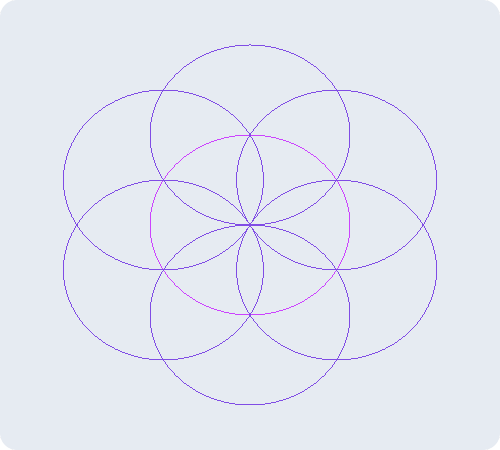
\includegraphics[width=17cm]{src/4.png}
\end{center}
\newpage


\Large{\textbf{Algoritmo de Traslación del Dibujo E}}\\[-0.5cm]
\begin{center}
\begin{mycodeboxl}
\begin{lstlisting}
from OpenGL.GL import *
from OpenGL.GLU import *
from OpenGL.GLUT import *
# Matriz de coordenadas del dibujo original
matriz_origen = [[100, 300, 200, 300, 200, 280, 100, 280],[100, 290, 130, 290, 130, 180, 100, 180],[100, 250, 160, 250, 160, 230, 100, 230],[100, 200, 200, 200, 200, 180, 100, 180]]
# Los componentes de esta matriz se sumarán a las cordenadas de la matriz de origen
matriz_traslacion = [200,0]

def dibujar_E():
    glBegin(GL_QUADS)
    glColor3f(0.8, 0.26, 1.0)
    glVertex2f(matriz_origen[0][0],matriz_origen[0][1])
    glVertex2f(matriz_origen[0][2],matriz_origen[0][3])
    glVertex2f(matriz_origen[0][4],matriz_origen[0][5])
    glVertex2f(matriz_origen[0][6],matriz_origen[0][7])

    glVertex2f(matriz_origen[1][0],matriz_origen[1][1])
    glVertex2f(matriz_origen[1][2],matriz_origen[1][3])
    glVertex2f(matriz_origen[1][4],matriz_origen[1][5])
    glVertex2f(matriz_origen[1][6],matriz_origen[1][7])
\end{lstlisting}
\end{mycodeboxl}
\end{center}
\newpage

\begin{center}
\begin{mycodeboxl}
\begin{lstlisting}
    glVertex2f(matriz_origen[2][0],matriz_origen[2][1])
    glVertex2f(matriz_origen[2][2],matriz_origen[2][3])
    glVertex2f(matriz_origen[2][4],matriz_origen[2][5])
    glVertex2f(matriz_origen[2][6],matriz_origen[2][7])

    glVertex2f(matriz_origen[3][0],matriz_origen[3][1])
    glVertex2f(matriz_origen[3][2],matriz_origen[3][3])
    glVertex2f(matriz_origen[3][4],matriz_origen[3][5])
    glVertex2f(matriz_origen[3][6],matriz_origen[3][7])
    glEnd()

def dibujar_E_trasladado():
    glBegin(GL_QUADS)
    glColor3f (0.5 , 0.3 , 0.9)
    glVertex2f(matriz_origen[0][0] + matriz_traslacion[0],matriz_origen[0][1] + matriz_traslacion[1])
    glVertex2f(matriz_origen[0][2] + matriz_traslacion[0],matriz_origen[0][3] + matriz_traslacion[1])
    glVertex2f(matriz_origen[0][4] + matriz_traslacion[0],matriz_origen[0][5] + matriz_traslacion[1])
    glVertex2f(matriz_origen[0][6] + matriz_traslacion[0],matriz_origen[0][7] + matriz_traslacion[1])
\end{lstlisting}
\end{mycodeboxl}
\end{center}
\newpage

\begin{center}
\begin{mycodeboxl}
\begin{lstlisting}
    glVertex2f(matriz_origen[1][0] + matriz_traslacion[0],matriz_origen[1][1] + matriz_traslacion[1])
    glVertex2f(matriz_origen[1][2] + matriz_traslacion[0],matriz_origen[1][3] + matriz_traslacion[1])
    glVertex2f(matriz_origen[1][4] + matriz_traslacion[0],matriz_origen[1][5] + matriz_traslacion[1])
    glVertex2f(matriz_origen[1][6] + matriz_traslacion[0],matriz_origen[1][7] + matriz_traslacion[1])
    
    glVertex2f(matriz_origen[2][0] + matriz_traslacion[0],matriz_origen[2][1] + matriz_traslacion[1])
    glVertex2f(matriz_origen[2][2] + matriz_traslacion[0],matriz_origen[2][3] + matriz_traslacion[1])
    glVertex2f(matriz_origen[2][4] + matriz_traslacion[0],matriz_origen[2][5] + matriz_traslacion[1])
    glVertex2f(matriz_origen[2][6] + matriz_traslacion[0],matriz_origen[2][7] + matriz_traslacion[1])

    glVertex2f(matriz_origen[3][0] + matriz_traslacion[0],matriz_origen[3][1] + matriz_traslacion[1])
    glVertex2f(matriz_origen[3][2] + matriz_traslacion[0],matriz_origen[3][3] + matriz_traslacion[1])
    glVertex2f(matriz_origen[3][4] + matriz_traslacion[0],matriz_origen[3][5] + matriz_traslacion[1])
    glVertex2f(matriz_origen[3][6] + matriz_traslacion[0],matriz_origen[3][7] + matriz_traslacion[1])
    glEnd()

\end{lstlisting}
\end{mycodeboxl}
\end{center}
\newpage
Gráfico generado 
\begin{center}

\includegraphics[width=16cm]{src/3.png}
\end{center}
\newpage

\end{document}
